\section{Introduction}
\label{sec:introduction-mcf10}

There are a variety of possible applications for the model outlined in chapter \ref{cha:stamm}; examples include stem cell reprogramming (\cite{Armond:2013} contributions to which are discussed in Section \ref{cha:stem-cells}) and estrogen response of Breast cancer cell lines \citep{Casale:2013}. Othere examples include a transitions Here we consider a derivative of the human epithelial MCF10A cell line where the v-Src and estrogen receptor (ER) fusion is integrated; the new cell line is called MCF10A-Er-Src \citep{Hirsch:2010ec} (for brevity in the discussion that follows we will refere to these as MCF10A). The Src oncogene is activated by by addition of tamoxifen resulting in a rapid transformation of this system. Morphological changes on a cellular level are observed as early as $t=24$ (between $t=24-36h$) they show the ability to form colonies in soft agar \citep{Hirsch:2010ec} in this transformed state. Figure \ref{fig:exp-pics} shows images taken of one realisation of the experiment using a camera attached to a microscope; they are taken at $t= \lbrace 0, 24, 48 \rbrace$ hours at two different magnification levels ($10x$ and $20x$ as indicated on the figure). The top rows shows images taken after induction of tamoxifen and the bottom row shows a null where no tamoxifen is added (see below for details).

In this chapter we discuss one application of the two-step estimation pipeline of STAMM (see Section \ref{sec:estim-pipe}). We investigate the oncogenic transformation of an MCF10A cell line using  data obtained by performing RNA-Seq measurements. 

\section{Relevance}
\label{sec:relevance}

This is a very interesting system to consider mainly because it consists of only a single perturbation i.e. induction of the classical oncogene v-Src. Additionally it is an exceptionally fast transformation (between $t=24-36$ hours) and changes are morphological and can be observed under a microscope. Additional the initial state is a cell-line therefore tests or follow up experiments are easy to carry out; which can include verification of estimated parameters.

\section{Experimental design}
\label{sec:experimental-design}

The experiments were performed in MCF10A-Er-Src cells, a derivative of mammary epithelial cell line MCF10A containing an integrated fusion of the v-Src oncoprotein with the ligand binding domain of ER \citep{Hirsch:2010ec,Iliopoulos:2009do}. The cells were cultured in DMEM/F12 medium supplemented as described in \cite{Debnath:2003km}. The Src oncogene was induced by addition of $1 \mu M$ tamoxifen to a 70-80\% confluent population, and induced and uninduced samples were harvested at the indicated timepoints for RNA isolation. The RNA was isolated by the Trizol method, and prepared for sequencing by the Illumina RNA TruSeq sample protocol.

\begin{figure}
  \centering
  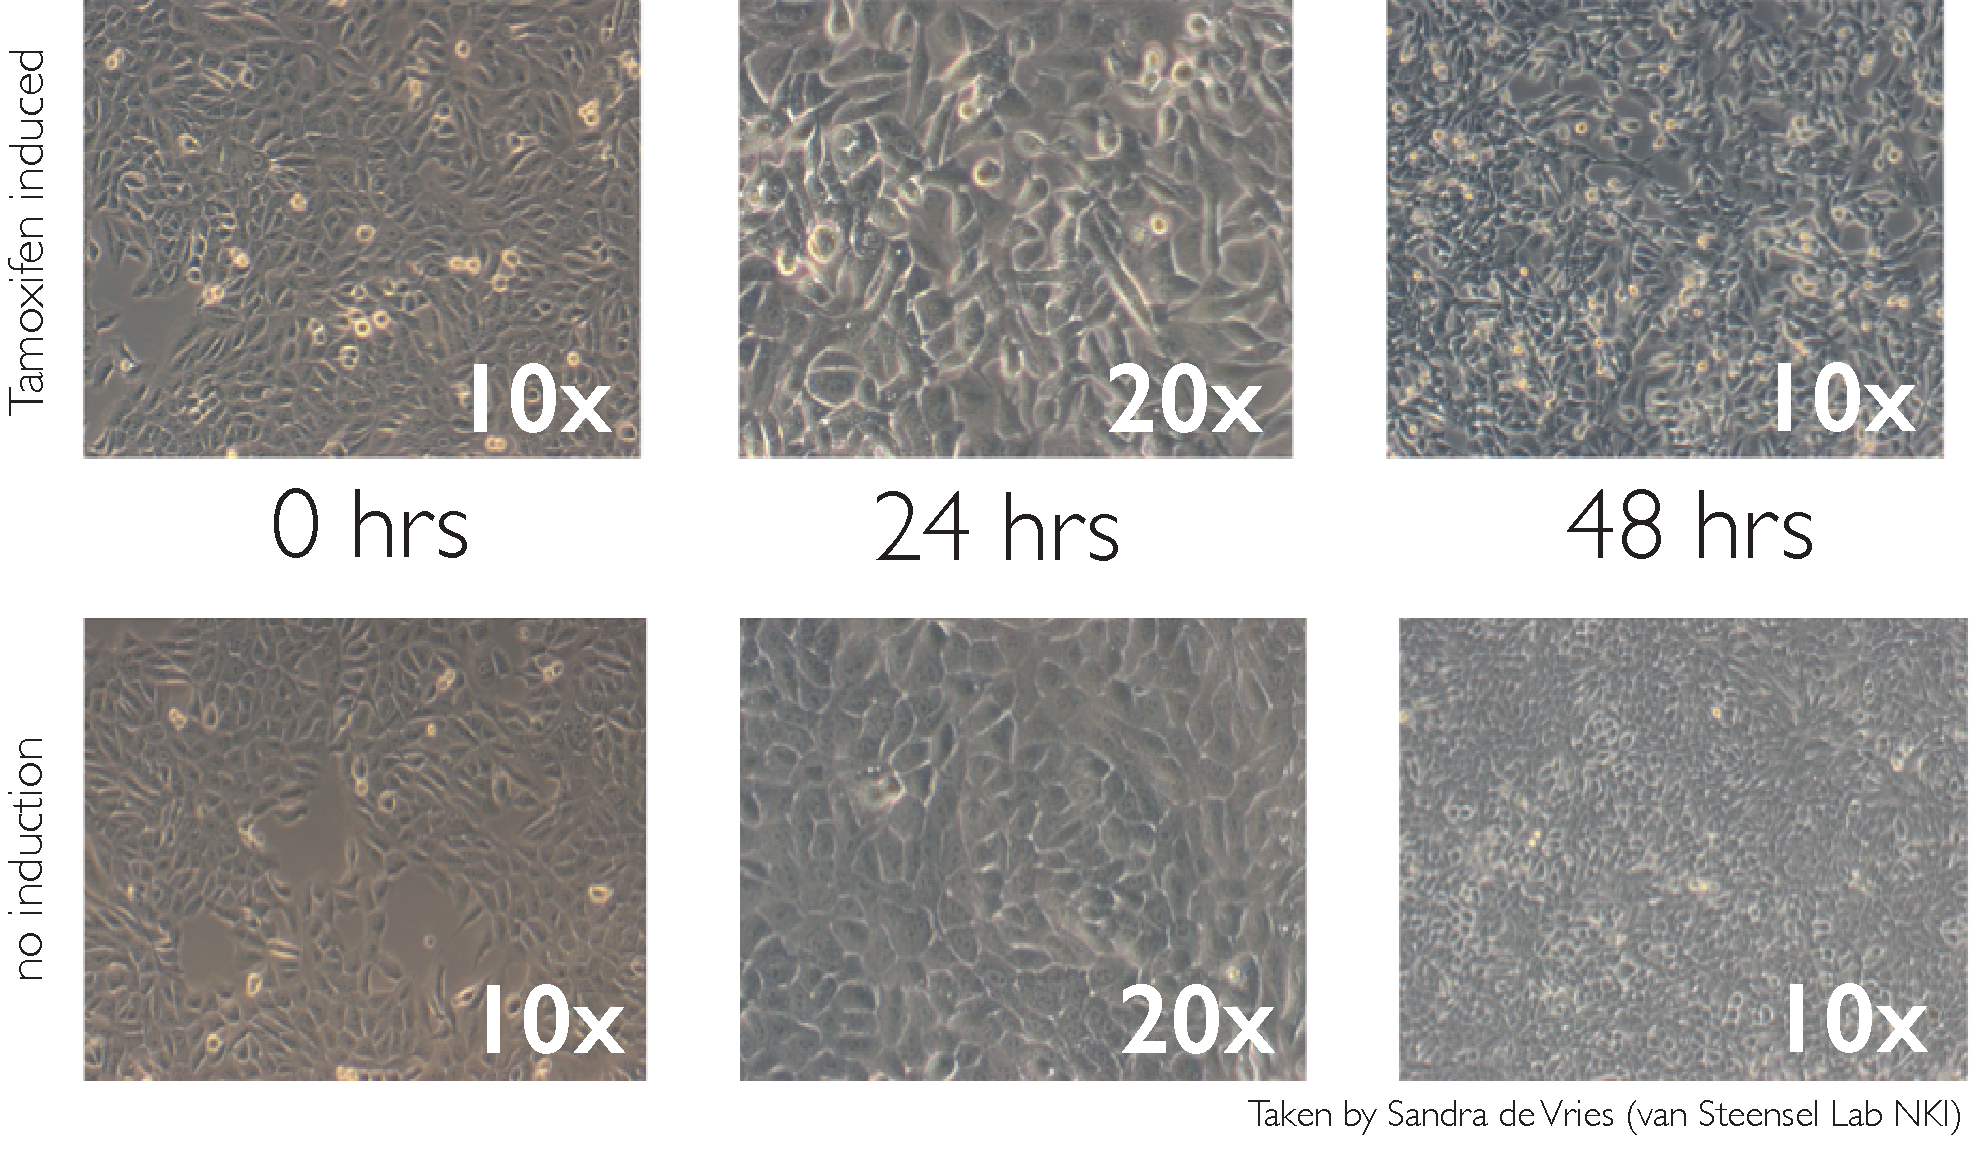
\includegraphics[width=1\textwidth]{pics/mcf10a-experiment}
  \caption{During the {\it in vitro} oncogenic transformation of an MCF10A-Er-Src cell line, morphological transformations can be observed between $24-36$ hours \citep{Hirsch:2010ec}. Here we show images taken of the experiment at three different time points. The initial measurement at $t=0$ hours and two subsequent measurements at $t=24$ and $t=48$ hours. The magnification each image is taken at is indicated on the images. The top row shows images of the experiment where Src is induced by addition of Tamoxifen at $t=0$; the bottom row shows images taken at the same time points without addition of Tamoxifen. It is possible to see morphological changes especially at $t=48$ where after addition of Tamoxifen cells are elongated.}
  \label{fig:exp-pics}
\end{figure}

\section{Pre-processing data}
\label{sec:norm-stand}

As described in Section \ref{sec:rna-sequencing} RNA-Seq data as obtained in this experiment is count data. 'Normalisation' is an important step when comparing samples in different settings {\color{red} change this}. Many methods exist to normalise sequencing experiments. We pre-process the data using the \texttt{edgeR} package in R \cite{McCarthy:2012wg,Robinson:2010cw}. One important assumption is that most genes are not differentially expressed between samples. To determine genes that are not differentially expressed the procedure uses a robust estimate for the ratio of RNA between samples a weighted trimmed mean of M values (TMM). Two parameters are employed to filter out genes that are differentially expressed; the M-values, log-fold-changes, and the A-value, absolute expression levels. The cut-off set for both the M-value and the A-value is tuneable and the best way to set the tuning parameters is to select a range of cut-off parameters and determining when they stabilise (see Section \ref{sec:sequencing-depth-rna}). It is important to remember \texttt{edgeR} was developed to analyse differential expression \cite{Robinson:2010dd}, still the assumptions are also applicable to time course such as the data set for the oncogenic transformation. Note without this step it is not possible to compare data from different samples.

After the first pre-processing step we still can't use the data in our model because the likelihood is based on an additive Gaussian noise model (eqn. (\ref{eq:likelihood})). For RNA-seq data once it has been 'normalised' the next pre-processing step is to transform the data such that distorting effects at high expression values are reduced. We use a nonlinear transform proposed by \cite{Hoffman:2012gn} the $\arcsinh x = \ln(x + \sqrt (x^2 + 1))$. The advantage of using this transformation compared to the more regularly used $\ln x$ is that it has the same effect at higher values but a much smaller effect at lower values. Now after applying these two pre-processing steps we can use this data in our model.

\section{Results}
\label{sec:results-mcf10a}

The data obtained uses RNA-seq to examine changes in gene expression during this transformation time-course with $T=13$ time points\footnote{$t=\lbrace 0, 0.5,  2,  4,  6,  8, 12, 16, 20, 24, 32, 40, 48h \rbrace$, at $t=0$ and $t=20$ we have a repeated measurements}. According to the assumption in our model all cells are in the initial state at $t=0$ are in an initial state. Here, by experimental design, the initial state consists of the derivative MCF-10A-Er-Src cell line. More specifically the time point $t=0$ in the here corresponds to the initial treatment with Tamoxifen an anti-oestrogen drug that binds to ER activating v-Src. Of course this is only the case excluding any unidentified epigenetic heterogeneity in the initial cell culture.  Therefore it is reasonable to assume that the cell population is approximately homogenous and comprised mainly of untransformed MCF-10A cells.


\begin{figure}
  \centering
  \includegraphics[width=0.7\textwidth]{pics/kmeans-dat.pdf}
  \caption{K-means clustering of {\it in vitro} data for the transformation of an MCF10A cell line. Initial k-means clustering is performed to identify representative trajectories. As described in Section \ref{sec:estim-pipe} we choose the optimal number of clusters $\hat{m}$ by considering relative changes in the objective function $\Delta J (m) = (J(m-1) - J(m))/J(m-1)$; we set $m$ where $\Delta J(m-1) < 0.1$. The plot shows $\Delta J$ as a function of $m$ and the horizontal dashed line represents our threshold at $0.1$. For this example we can see that the $\hat{m} = 13$. Note that fluctuation in $\Delta J$ at higher $m$ are due to small values of $J(m)$. }
  \label{fig:kmeans-dat}
\end{figure}


\begin{figure}
  \centering
  \includegraphics[width=0.8\textwidth]{pics/no-pen-data.png}
  \caption{The RNA-seq measurements are filtered with respect to standard deviation (we filter out genes with $\sigma_j > 20$ before transformation) because we are interested in genes that change significantly in time. Test stability of estimates to determine need for penalisation.}
  \label{fig:data-pen}
\end{figure}

To focus 
on genes that change over time  during transformation we filtered  genes $j$ with respect to 
 standard deviation $\sigma_j$, retaining genes with $\sigma_j > 20$ (on the linear scale, over time). 
This gave a set of $p=2809$ gene expression trajectories to which STAMM was applied. 
Estimation was carried out 
following the  pipeline described in Methods, including 
an initial test of the need for penalization (penalization was not needed; see Fig 7(b) SI). 
We used  two-stage estimation (see Methods), 
clustering the data 
to obtain representative centroids from which to estimate transition rates (Fig 8 SI), and using $\arcsinh$
as the transformation function $g$. 
The proposed cross-validation-based model selection score showed a minimum at $K=4$ states (Fig. \ref{fig:data_fit}(a)).
This suggests that oncogenic transformation of the MCF-10A cells occurs via four transcriptionally-distinct states. A representative set of trajectories and corresponding fitted model output are shown in Fig. \ref{fig:data_fit}(b) with corresponding 
state-specific gene expression parameters $\beta_j$ shown in Fig. \ref{fig:data_fit}(c).
Finally, we carried out a post-estimation diagnostic of sensitivity to the tuning parameter $m$ (number of initial clusters);
Fig. \ref{fig:data_fit}(d) shows the correlation between reported $\beta$'s and those obtained with increasing $m$; we find that the estimates are not sensitive to choice of $m$.

\begin{figure}
  \centering
  \subfigure[Number of state $K$]{
    \includegraphics[width=0.45\textwidth]{pics/loocv-dat.pdf}
  }
  \subfigure[Stability of number of cluster]{
    \includegraphics[width=0.45\textwidth]{pics/stab-m-dat.pdf}
  }
    \caption{Determining number of states $K$ and stability test}
  \label{fig:data-m-k}
\end{figure}

The foregoing example illustrates the application  of the proposed methods to genome-wide RNA-seq data, including empirical diagnostics. However, investigation and validation of these potentially novel states is beyond the scope of the present paper (see also Discussion below).

%%% Local Variables:
%%% TeX-master: "warwickthesis"
%%% End:
